\chapter{Systèmes nucléon-nucléon}
\section{Formalisme de l'isospin}
	\subsection{Définition}
	Basé sur l'évidence relative que le proton et le neutron sont semblables, \textsc{Heisenberg} 
	introduit le formalisme de l'\textbf{isospin} en \textit{1932}. Parmi les ressemblances, on retrouve
	\begin{itemize}
	\item[$\bullet$] Différence de 0.14\% entre les masses : $m_n = 939.57$ MeV et $m_p = 938.27$ MeV
	\item[$\bullet$] Symétrie de charge $V_N^{pp} \approx V_{N}^{nn}$
	\item[$\bullet$] Indépendance de la charge $V_N^{pp} \approx V_{N}^{nn} \approx V_{N}^{np}$
	\end{itemize}
	Nous parlons bien évidemment ici des interaction coulombiennes. L'idée est alors de voir le
	\textbf{nucléon} comme une seule particule avec un isospin $t=1/2$. Il existe alors deux 
	projections possibles, soit deux états possibles (d'une même particule)(fonction de la charge)
	\begin{equation}
	m_t = \frac{1}{2} \text{pour le neutron} = \ket n = \left(\begin{tabular}{c}
	1\\
	0
	\end{tabular}\right),\qquad 	m_t = -\frac{1}{2} \text{pour le proton} = \ket n = \left(\begin{tabular}{c}
	0\\
	1
	\end{tabular}\right)
	\end{equation}
	On dénombre ainsi trois opérateur d'isospin
	\begin{equation}
	\vec{t} = (t_x,t_y,t_z)
	\end{equation}
	L'isospin n'est rien autre qu'un nouveau moment cinétique lié à la charge
	\begin{equation}
	\hat{q} = e\left(\dfrac{1}{2}-t_z\right)
	\end{equation}
	Il vérifie donc les relation habituelles des moments cinétiques
	\begin{equation}
	t_z\ket n = \frac{1}{2}\ket n,\qquad t_z\ket p = -\frac{1}{2}\ket p,\qquad \vec{t}^2\ket n = \frac{3}{4}
	\ket n,\qquad \vec{t}^2\ket p = \frac{3}{4}\ket p
	\end{equation}
	On peut également définir des opérateurs élévateurs ($t_+ = t_x+it_y$) et abaisseurs ($t_- = t_x-it_y$)
	qui seront utile\footnote{Avec $t_+\ket p = \ket n$ et $t_+\ket n = 0$.} dans le cadre de la radioactivité
	 $\beta$ où un neutron est transformé en proton et inversement. \\
	 
	Notons que le concept d'isospin est plus général que le nucléon, on peut en parler dans d'autres types de
	particules (pion ou l'on associe un isospin $t$ de 1).

	\subsection{Isospin du noyau}
	Considérons un noyaux de $Z$ protons et $N$ neutrons tel que $Z+N=A$. L'\textbf{isospin total} est 
	le couplage des $A$ moments cinétiques
	\begin{equation}
	\vec T = \sum_{i=1}^A \vec t_i
	\end{equation}
	
	\notes{Soit $\vec J = \vec j_1 + \vec j_2 \to M = M_1 + M_2$, les projections. On a alors
	\begin{equation}
	\begin{array}{ll}
	\vec{j_1}^2\ket{j_1m_1} = j_1(j_1+1)\ket{j_1m}\\
	\vec{J}^2\ket{JM} = J(J+1)\ket{JM}
	\end{array},\qquad -j_1\leq m \leq j_1\quad \text{(projection)}
	\end{equation}
	où\\
	
	\cadre{\begin{equation}
	|j_1-j_2| \leq J \leq j_1+j_2\qquad\text{et}\qquad M=m_1+m_2	
	\end{equation}}\ \\
	
	Pour l'isospin, nous avons $t_z=1/2$ (neutron) et $t_z=-1/2$ (pronton) et donc\\
	
	\cadre{\begin{equation}
	T_z = N\frac{1}{2} + Z\left(-\frac{1}{2}\right) = \dfrac{N-Z}{2}
	\end{equation}}}\ \\
	
	Les valeurs propres sont alors données par $T_z = \dfrac{N-Z}{2}$ et en comme dans la plupart des
	noyaux $N>Z$ on en tire que
	\begin{equation}
	\left|\dfrac{N-Z}{2}\right| \leq T \leq \dfrac{N+Z}{2}
	\end{equation}
	Ainsi, dans le fondamental nous avons presque toujours $T=\left|\dfrac{N-Z}{2}\right|$. Un atome 
	de masse $A$ paire aura alors $T$ entier et $A$ impaire implique $T$ demi-entier.\\
	
	

	\begin{wrapfigure}[12]{r}{5cm}
	\vspace{-5mm}
	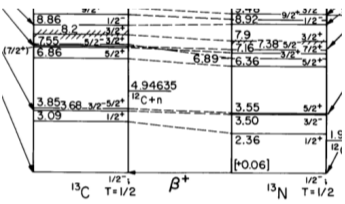
\includegraphics[scale=0.45]{ch2/image1.png}
	\captionof{figure}{ }
	\end{wrapfigure}
	\textsc{Intérêt expérimental}\\
	Les noyaux miroirs sont des noyaux tel que l'on a $(Z_1,N_1)$ et $(Z_2=Z_1, N_2=N_1)$, impliquant 
	des spectres très similaires. L'isospin permet de les différencier. Par exemple $\ ^{13}C$ possède 6 protons 
	et 7 neutrons mais un isospin $T_z=+1/2$ tandis que le $\ ^{13}N$ possède 7 protons et 6 neutrons et 
	un isospin $T_z= -1/2$.\\
	
	\subsubsection{Hamiltonien du noyau (formalisme de l'isospin)}
	Dans ce formalisme, l'hamiltonien s'écrit
	\begin{equation}
	H = sum_i T_i + \sum_{i<j} V_N(i,j) + \sum_{i<j} V_C(i,j)
	\end{equation}
	où le premier terme est l'énergie cinétique $T$
	\begin{equation}
	T_i = \frac{p_i^2}{2m_N}=\frac{-\hbar^2}{2m_N}\Delta_t,
	\end{equation}
	le second terme est le potentiel nucléaire indépendant de $T$
	\begin{equation}
	[V_n,T]=0
	\end{equation}
	et le dernier terme est le potentiel coulombien (commun à tous les électrons), qui peut être écrit
	de façon tout à fait générale grâce à l'isospin.
	\begin{equation}
	V_C(i,j) = \frac{e^2}{|r_i-r_j|}\left(\frac{1}{2}-t_{iz}\right)\left(\frac{1}{2}-t_{jz}\right),\qquad
	[V_C,T_z]=0,\qquad [V_C, T^2]\neq 0
	\end{equation}		
	Le premier commutateur implique que $T_z$ est un \textit{bon} nombre quantique mais le second montre que
	$T$ n'est pas rigoureusement un bon nombre quantique. \\
	
	\notes{Quelques petites remarques\ 
	\begin{itemize}
	\item[$\bullet$] $[H,J^2]=0$ implique la quantification des niveaux d'énergie
	\item[$\bullet$] $[H,P]=0$ implique que chaque niveau est soit +1, soit -1
 	\item[$\bullet$] $[H,T^2]\approx0$ implique un nombre quantique approximatif et pas d'état strict d'isospin
	\end{itemize}
	La première séance d'exercice nous illustre le calcul de $T_z$. Le principal intérêt de cette notion est
	dès lors bien de classifier les différents niveaux d'énergie\footnote{Voir slide 22 pour s'en convaincre.}}

	
\section{Le deuton}
Le deuton est un système lié formé d'un neutron et d'un proton où $T_z=0$, soit un isotope lourd de l'hydrogène.
Théoriquement  $J$ peut alors valoir 0 ou 1 mais de expérimentalement on ne trouve que la valeur non-nulle. 
Les mesures expérimentales sont les suivantes
\begin{equation}
E_B = 2.224\ \text{MeV},\qquad J=1^+,\qquad \sqrt{\langle r^2\rangle}\approx 2.1\ \text{fm}, \qquad Q=
0.286\ \text{e.fm$^{2}$}
\end{equation}
où $Q$ est le \textbf{moment quadripolaire}. Celui-ci est lié à la déformation du noyau (seulement les 
protons) et se défini
\begin{equation}
Q_{2\mu} = e\sum_{i=1}^Z r_i^2Y_2^\mu(\Omega_i) = e\sum_{i=1}^A \left(\frac{1}{2}-t_{iz}\right)r_i^2
Y_2^\mu(\Omega_i)
\end{equation}
Il s'agit d'un OTI de rang 2 vis-à-vis de $l$. Nous y reviendrons plus tard. Intéressons-nous d'abord 
aux nombres quantiques. Vu les résultats expérimentaux, il faut trouver une combinaison donnant $1^+$.
\begin{equation}
\begin{array}{lll}
S = S_p+S_n\qquad&\to s=0\quad &\leftrightarrow L=1\\
&\to s=1&\leftrightarrow L=0,1,2
\end{array}
\end{equation}
La parité calculée via $(-1)^L$ exclu la valeur $L=1$, seules les valeurs $L=0,2$ sont possibles (et $L=0$ 
est dominant). Le deuton correspond alors aux valeurs $S=1$ et $L=0,2$.\\

En partant de la relation d'incertitude $\Delta p\Delta x = \hbar = 197$ MeV.fm, pour $\Delta x\approx$ 
1 fm on trouve $\Delta p \approx 200$ MeV/c. L'énergie cinétique vaut donc 
\begin{equation}
T \approx \dfrac{(\Delta p)^2}{2m_N} = \dfrac{4*10^4}{2*10^3} \approx 20\text{ MeV}
\end{equation}
Ce qui est l'énergie cinétique par nucléon. Cette énergie étant faible par rapport à l'énergie de masse du 
nucléon ($m_Nc^2$), on utilisera l'équation de \textsc{Newton} mais il faut bien garder à l'esprit qu'il
faudrait utiliser l'équation de \textsc{Dirac} dans un régime relativiste. L'énergie vaut donc
\begin{equation}
E = \underbrace{T}_{\approx 20\text{ MeV}} + \underbrace{V}_{\approx -22\text{ MeV}} = -2.2\ \text{MeV}
\end{equation}
où le potentiel est attractif. L'état est donc un état lié. Il est possible de calculer via l'expression 
de la vitesse $v= \Delta p/m_N\approx c/5$ un temps caractéristique pour une distance de 5 fm de $10^{-22}$ s.
	
	
	
	
\section{Systèmes de deux nucléons}
La première chose à faire lorsqu'on s'intéresse aux propriétés nucléaires et de regarder les symétries. Sachant
que les nucléons sont des fermions, la fonction d'onde totale doit être antisymétrique : $P_{12}\Psi = -\Psi$
où $P_{12}$ est l'opérateur d'échange des coordonnées spatiales, de spin et d'isospin. Il est possible 
d'utiliser une factorisation de ces trois composantes
\begin{equation}
\Psi_{LST}(\vec{r}) = \Phi_L(\vec{r})\ket{SM_S}\ket{TM_T}
\end{equation}
On utilisera alors le moment cinétique orbital relatif $\vec{L}$, le spin total $\vec{S}=\vec{S_1}+\vec{S_2}$ 
et l'isospin total $\vec T = \vec T_1+\vec{T_2}$. Deux cas sont possibles
\begin{enumerate}
\item Pour $S=1$, il s'agit de l'état \textit{triplet} aux fonctions d'ondes symétriques
\item Pour $S=0$, il s'agit de l'état \textit{singlet} aux fonctions d'ondes antisymétriques
\end{enumerate}
Si on définit $P^\sigma$ comme l'opérateur d'échange des spins\footnote{Il s'agit d'une notation historique 
où $\sigma=2S$.}, on a
\begin{equation}
P^\sigma\ket{SM_S} = (-1)^{S+1}\ket{SM_S}
\end{equation}
Le tout est maintenant de trouver une expression analytique de cet opérateur, qui possède les valeurs propres
$(-1)^{S+1}$. Pour se faire, considérons le produit scalaire suivant : $\vec s_1.\vec{s_2} = 1/2(
\vec{S}^2-\vec s_1^2-\vec s_2^2)$. On en tire
\begin{equation}
\begin{array}{ll}
\vec s_1.\vec s_2\ket{S=0, M_S=0} &=\DS \frac{1}{2}\left(0-\frac{3}{4}-\frac{3}{4}\right)\ket{S=0,M_S=0} = 
\frac{-3}{4}\ket{0,0}\vspace{2mm}\\
\vec s_1.\vec s_2\ket{S=0, M_S} &=\dfrac{1}{4}\ket{1,M_S}
\end{array}
\end{equation}
	
On en tire que (rouge)
\begin{equation}
P^\sigma = \frac{1+4\vec s_1\vec s_2}{2} = \frac{1+\vec\sigma_1\vec\sigma_2}{2}
\end{equation}		
où $\sigma = 2s$. On a bien un opérateur donnant la phase recherchée. En effet, l'application de $P^\sigma$ à 
une fonction $S=0,1$ donne une phase lisse. Ce qui a été fait pour le spin peut évidemment se faire pour l'isospin,
c'est la même chose
\begin{equation}
P^\tau = \dfrac{1+\vec\tau_1\vec\tau_2}{2}
\end{equation}

Ceci était pour l'échange de spin (et isospin). Nous avons également l'\textbf{opérateur d'échange des 
coordonnées d'espaces} défini selon
\begin{equation}
P^r\Phi_L(\vec{r}) = \Phi_L(-\vec{r})=(-1)^L\Phi_L(\vec{r})
\end{equation}

Pour échanger deux nucléons (espace, spin, isospin), on utilisera alors
\begin{equation}
P_{12} = P^rP^\sigma P^\tau
\end{equation}

\newpage


	\begin{wrapfigure}[7]{l}{9cm}
	\vspace{-1mm}
	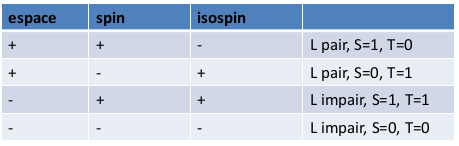
\includegraphics[scale=0.5]{ch2/image2}
	\captionof{table}{ }
	\end{wrapfigure}

Étant des fermions, les nucléons possèdent une fonction d'onde antisymétrique. Il faut que $P_{12}\psi = -\psi$. 
On en tire le \textbf{principe de Pauli généralisé} (rouge) :
\begin{equation}
P_{12} = P^rP^\sigma P^\tau = -1
\end{equation}
En effet, l'application de $P_{12}$ sur $\psi$ où $\psi$ est caractérisé par quatre nombres quantiques $L,S,T$ donne
\begin{equation}
(-1)^S+1 (-1)^T+1 (-1)^L = -1
\end{equation}
Et donc
\begin{equation}
(-1)^{L+S+T} =-1
\end{equation}
Il s'agit d'une \textbf{règle de sélection pour le système nucléon-nucléon}. \\


	\begin{wrapfigure}[6]{r}{9cm}
	\vspace{-1mm}
	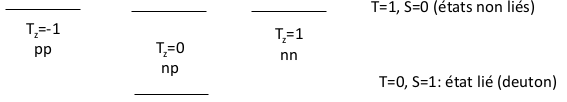
\includegraphics[scale=0.5]{ch2/image3}
	\captionof{figure}{ }
	\end{wrapfigure}
Ainsi, en parité + ($L$ pair), on dénombre quatre états. Le cas $T=1,S=0$ sont des états non liés alors
que $T=0, S=1$ forme un état lié (deuton). En parité - ($L$ impair), on compte quatre états non liés.
	
	
	
\section{Interaction nucléon-nucléon}
Aujourd'hui encore, cette interaction n'est pas exactement connue. Ce que l'on sait, c'est qu'elle doit 
respecter six \underline{lois d'invariances}
\begin{enumerate}
\item Réflexion
\item Translation (dépend de $\vec{r}=\vec r_1-\vec r_2, \vec p = \vec p_1-\vec p_2$)
\item Rotation
\item Invariance par rapport au temps
\item Indépendance de charge
\item $V(1,2)=V(2,1)=V(r_1,r_2;p_1,p_2;s_1,s_2;t_1,t_2)$
\end{enumerate}\ \\

De même, le \underline{principe de Pauli généralisé} doit s'appliquer
\begin{equation}
P_{12}\Psi_{LST}(\vec{r}) = -\Psi_{LST}(\vec{r})
\end{equation}
où $P_{12}=P^rP^\sigma P^\tau$. On donne une forme générale au potentiel $V(r)$
\begin{equation}
V(r) = w(r)+m(r)P^r+b(r)P^\sigma + h(r)P^\tau
\end{equation}
où l'on part de données expérimentales ($B, Q, \mu$, déphasages, \dots) et on ajuste ces fonctions selon les
données mesurées. Encore une fois, l'interaction nucléon-nucléon est non-connue, il n'existe que des formes 
que les gens ont ajustés. Souvent, on utilise des formes soit Gaussiennes, soit de \textsc{Woods-Saxon}.\\


Voyons comment faire. Considérons un \underline{système n+p $(T_z=0)$} où $L$ est pair. En considérant la
forme générale du potentiel (central) $V(r) = w(r)+m(r)P^r+b(r)P^\sigma + h(r)P^\tau$, on trouve comme
éléments de matrice
\begin{equation}
\begin{array}{ll}
\bra{T=0S=1}V\ket{T=0,S=1} &= w(r)+m(r)+b(r)-h(r)\\
\bra{T=1S=0}V\ket{T=1,S=0} &= w(r)+m(r)-b(r)+h(r)
\end{array}
\end{equation}
On peut déjà remarquer que l'on obtient des potentiels différents pour $S=0$ (singlet) et $S=1$ (triplet). 
\begin{center}
		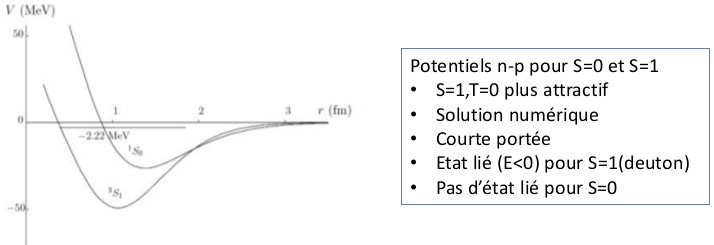
\includegraphics[scale=0.6]{ch2/image4}
	\captionof{figure}{ }
	\end{center}
	
Pour un \underline{système	 $n+n\ (T_z=+1), p+p (T_z=-1)$}, $L$ pair ($T=0\nexists$)
\begin{equation}
\bra{T=1S=0}V\ket{T=1,S=0} = w(r)+m(r)-b(r)+h(r)
\end{equation}
Comme on retrouve le même potentiel pour les trois systèmes $T=1$, il y a invariance de la charge. Dans une
interaction centrale, on peut donc dire que $\Delta S= 0$ et $\Delta L = 0$.\\

Il est possible de prendre en comptes des \underline{termes additionnels} dans l'interaction nucléon-nucléon
(couplage spin-orbite, terme tensoriel, \dots). On pourrait avoir \textit{par réflexion}
\begin{equation}
(\vec r, \vec p, \vec s_1, \vec{s_2}) \to (-\vec r, -\vec p, \vec s_1, \vec{s_2})
\end{equation}
Par \textit{renversement du temps}
\begin{equation}
(\vec r, \vec p, \vec s_1, \vec{s_2}) \to (\vec r, -\vec p, -\vec s_1, -\vec{s_2})
\end{equation}	

On pourrait aussi rajouter des termes "non-centraux" comme le \textit{spin-orbite}
\begin{equation}
V_{LS}(r)\vec{L}.\vec{S} \qquad :\qquad \Delta S =0,\pm 1, \Delta L = 0
\end{equation}
où encore des termes \textit{tensoriels}
\begin{equation}
V_T(r)\vec{S}_{12}\qquad \text{avec }\quad \vec{S_{12}} = [[\vec{s_1}\otimes \vec{s_2}]^2\otimes
[\vec{r_1}\otimes \vec{r_2}]^2]^0
\end{equation}
Ce terme respecte également les propriétés d'invariances énoncées ci-dessus. Il est responsable d'un
mélange entre $L=0$ et $M=2$ dans le deuton, mais également du moment quadrupolaire du deuton.\\

L'interaction nucléon-nucléon n'est pas exacte, mais ajustée. Si on utilise cette expression pour un 
système à trois corps, on ne trouve pas exactement la valeur expérimentale de l'énergie. C'est parce que,
pour des systèmes nucléaires à trois corps, il existe des forces à trois corps :
\begin{equation}
H = T_1+T_2+T_3 + V_{12}+V{13}+V{23}+V{123}
\end{equation}